\section{The diodes bridge example}

\begin{figure}[h]
\centerline{
 \scalebox{0.7}{
    \input{Bridge.pstex_t}
 }
}
 \caption{Diodes bridge}
\label{fig-Diode-bridge}
\end{figure}




\subsection{Unknowns}

x = $^{t}(U_{1},I_{7})$,
$Z_{ns}=^{t}(I_{2},I_{3},I_{4},I_{5}$),
$Z_{s} = ^{t}(V_{1},V_{2},V_{3})$
\subsection{Diode non smooth model instance}

\[ z_{i} = I_{i}\]
\[ \alpha =U_{i}\]
\[z_{i}=1l_{i}+0\alpha\]
\[y_{i}=1\alpha+0l_{i}\]
\[0 \leq y_{i} \, \perp \, l_{i} \geq 0\]


\subsection{Global formulation}

\[ \lambda =(l_{1},l_{2},l_{3},l_{4})\]
\[Z_{ns}=0X+0Z_{s}+Id\lambda\]
\[Y=\left(\begin{array}{cc}
0&0\\
0&0\\
0&0\\
0&0\end{array}\right) x+
\left(\begin{array}{ccc}
0&1&0\\
0&0&1\\
1&0&-1\\
1&-1&0\end{array}
\right) Z_{s} + 0Z_{ns} +0\lambda\]

\[0 \leq Y \, \perp \, \lambda \geq 0\]

Note that :
\begin{itemize}

  \item[--] The diode 2 is managed by the couple $(l_1,y_1)$
  \item[--] The diode 3 is managed by the couple $(l_2,y_2)$
  \item[--] The diode 4 is managed by the couple $(l_3,y_3)$
  \item[--] The diode 5 is managed by the couple $(l_4,y_4)$
\end{itemize}
\subsection{Matrices formulation}
\[
\left(\begin{array}{c}
  
x'=\left(\begin{array}{cc}
0 &\frac{-1}{C}\\
0&0\end{array} \right)x
+\left(\begin{array}{ccc}
0&0&0\\
\frac{1}{L}&0&0\end{array} \right)Z_{s}
+\left(\begin{array}{cccc}
0&0&\frac{1}{C}&\frac{-1}{C}\\
0&0&0&0\end{array} \right)Z_{ns}
\\
0=\left(\begin{array}{cc}
0 &0\\
0 &0\\
1 &0\end{array} \right)x
+\left(\begin{array}{ccc}
0&\frac{1}{R}&\frac{-1}{R}\\
0&\frac{-1}{R}&\frac{1}{R}\\
0&1&0\end{array} \right)Z_{s}
+\left(\begin{array}{cccc}
1&0&0&1\\
0&+1&1&0\\
0&0&0&0\end{array} \right)Z_{ns}
\\
Z_{ns}=Dx+0Z_{s}+Id\lambda\\
Y=0x+
\left(\begin{array}{ccc}
0&1&0\\
0&0&1\\
1&0&-1\\
1&-1&0\end{array}
\right) Z_{s} + 0Z_{ns} +0\lambda\\

0 \leq Y \, \perp \, \lambda \geq 0

\end{array}
\right)
\]
The first is the KCL at the node 1.\\
The second line is the inductor law.\\
The third line is the KCL at the node 3.\\
The fourth line is the KCL at node 2.\\
The fifth line is $U_1 + V_1=0$.\\

\subsection{Simulation}
C= 1 uF\\
L= 10 mH\\
R= 1000 $\ohm$\\
The simulation computed 450 steps with a 10 $\micro$s fixed time step. The figure
\ref{fig-Diode-sim} shows the tension in the resistor branch.


\begin {figure}[h]
%GNUPLOT: LaTeX picture with Postscript
\begin{picture}(0,0)%
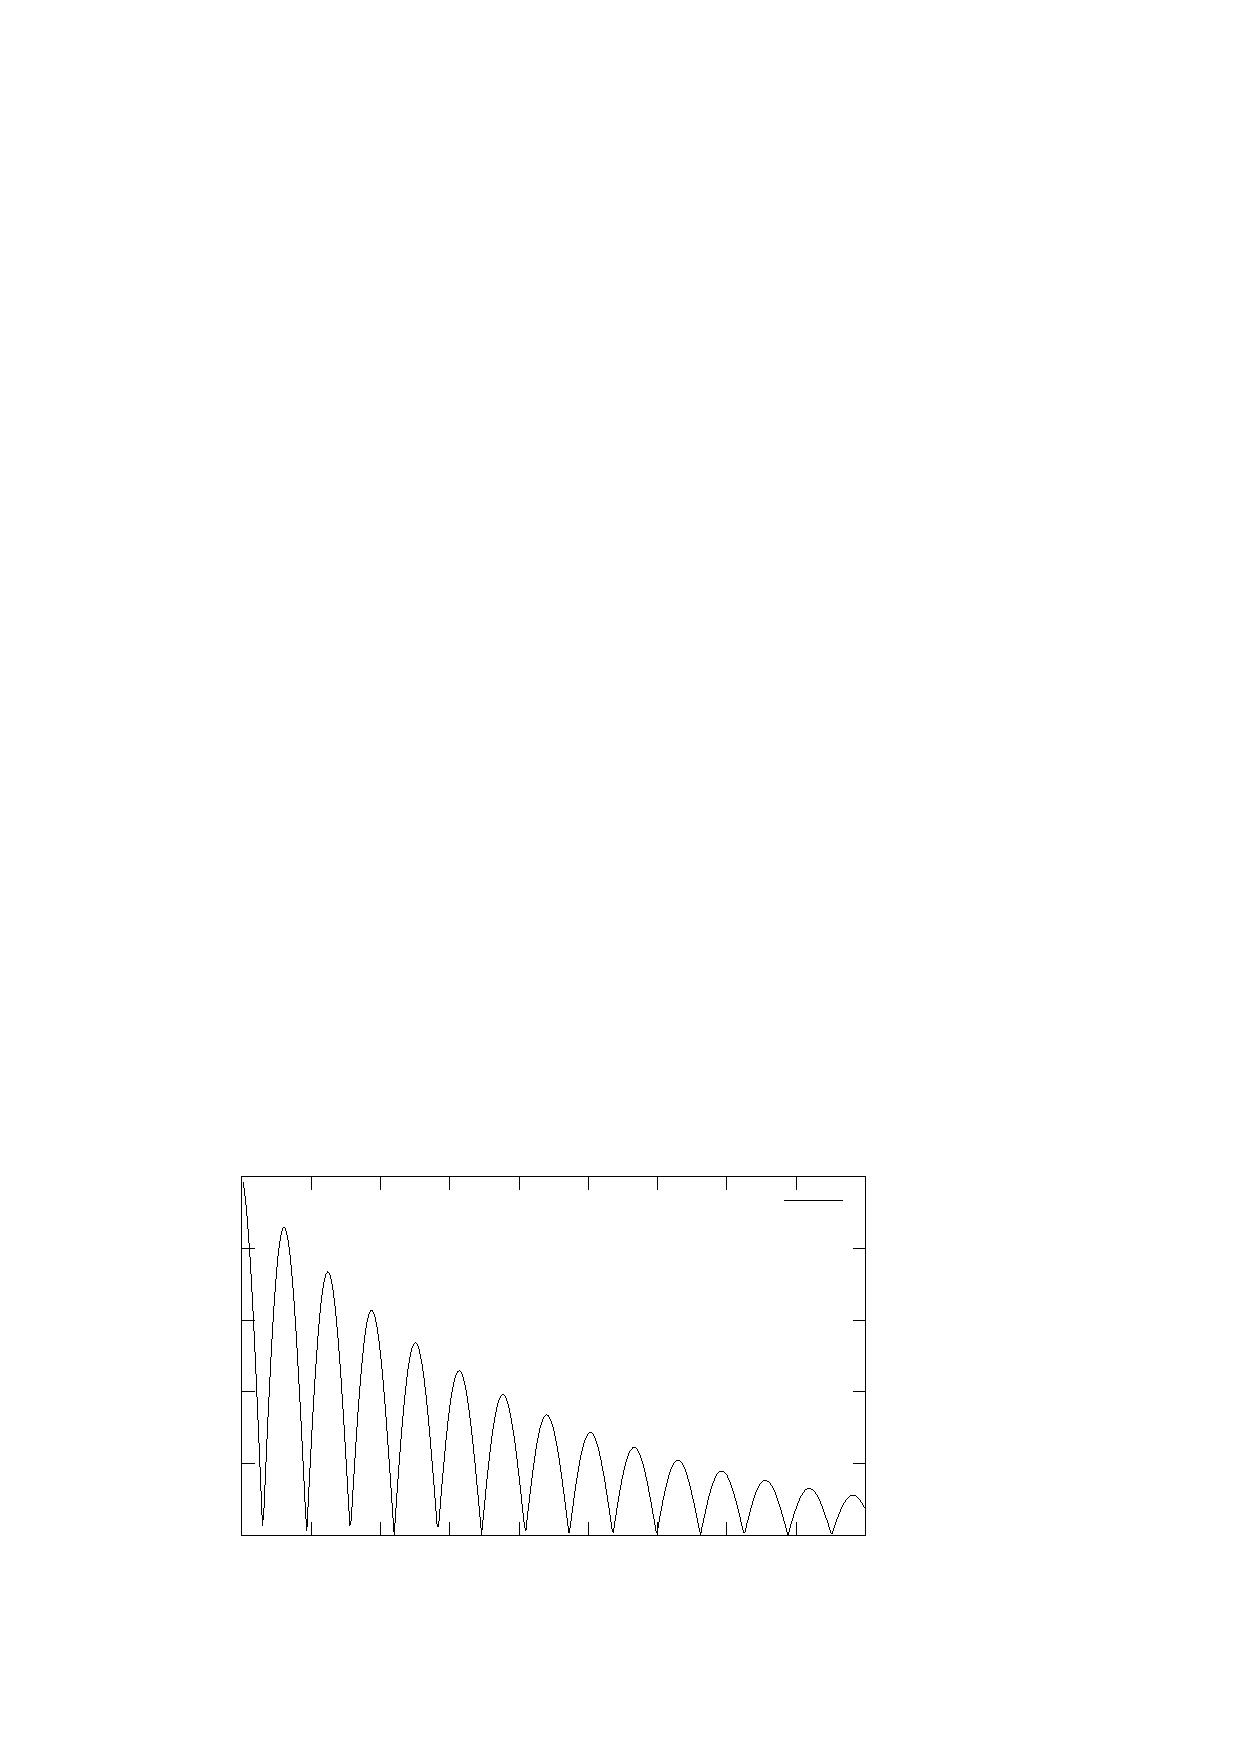
\includegraphics{diodes}%
\end{picture}%
\begingroup
\setlength{\unitlength}{0.0200bp}%
\begin{picture}(18000,10800)(0,0)%
\put(1925,1650){\makebox(0,0)[r]{\strut{} 0}}%
\put(1925,3370){\makebox(0,0)[r]{\strut{} 2}}%
\put(1925,5090){\makebox(0,0)[r]{\strut{} 4}}%
\put(1925,6810){\makebox(0,0)[r]{\strut{} 6}}%
\put(1925,8530){\makebox(0,0)[r]{\strut{} 8}}%
\put(1925,10250){\makebox(0,0)[r]{\strut{} 10}}%
\put(2200,1100){\makebox(0,0){\strut{} 0}}%
\put(3864,1100){\makebox(0,0){\strut{} 50}}%
\put(5528,1100){\makebox(0,0){\strut{} 100}}%
\put(7192,1100){\makebox(0,0){\strut{} 150}}%
\put(8856,1100){\makebox(0,0){\strut{} 200}}%
\put(10519,1100){\makebox(0,0){\strut{} 250}}%
\put(12183,1100){\makebox(0,0){\strut{} 300}}%
\put(13847,1100){\makebox(0,0){\strut{} 350}}%
\put(15511,1100){\makebox(0,0){\strut{} 400}}%
\put(17175,1100){\makebox(0,0){\strut{} 450}}%
\put(550,5950){\rotatebox{90}{\makebox(0,0){\strut{}U23}}}%
\put(9687,275){\makebox(0,0){\strut{}time e-5 s}}%
\put(14950,9675){\makebox(0,0)[r]{\strut{}'DiodeBridge.traj'}}%
\end{picture}%
\endgroup
\endinput

\caption{Diode bridges simulation}
\label{fig-Diode-sim}
\end {figure} 
